
In this chapter, we will review the basic concepts of the physics of a particle trapped in a periodic potential. This will set the stage for extending our formalism to the many-particle system of bosons that we wish to study in this thesis. 

\section{Exploiting structure}
Consider a particle of mass $m$ trapped in a 1D periodic potential $V(x)$ with period $a$. The Hamiltonian can then be written as:
\begin{equation}
    \hat{H} = \frac{\hat{p}^2}{2m} + \hat{V}(x)  \hspace{1cm} V(x + a) = V(x)    
\end{equation}
In an attempt to uncover some structure in this system, let us draw a parallel with the special case of a free-particle where $V(x) = 0$. Such a system has a continuous translation symmetry, i.e, $V(x + a) = V(x) \hspace{0.1cm}\forall a$. As a result of Noether's theorem, the momentum $k$ is a conserved quantity and hence a good quantum number to label the eigenstates. 
\vspace{0.5cm}\\
However, in the case of a periodic potential, the system only has a discrete translation symmetry. Equivalently, the Hamiltonian commutes with the translation operator, $\hat{T}_a = e^{-i\hat{p}a/\hbar}$:
\begin{equation}
    \hat{T}_a \hat{H}\hat{T}_a^{-1} = \hat{H} \hspace{0.5cm}\Longleftrightarrow \hspace{0.5cm}[\hat{T_a}, \hat{H}] = 0
\end{equation}
We can then find the common eigenbasis of $\hat{H}$ and $\hat{T}_a$:
\begin{equation}
    \hat{H}\psi_{E, \alpha}(x) = E\psi_{E, \alpha}(x) \hspace{1cm}\hat{T}_a\psi_{E, \alpha}(x) = \psi_{E, \alpha}(x+a) = e^{i\alpha}\psi_{E, \alpha}
\end{equation}
where the eigenvalues of $\hat{T}_a$ must be pure phases since it is a unitary operator. Now consider the following function $u_{E, \alpha}(x) = e^{-iqx}\psi_{E, \alpha}(x)$ and its behaviour under the action of $\hat{T}_a$:
\begin{align*}
    \hat{T}_a u_{E, \alpha}(x) &= \hat{T}_a e^{-iqx} \psi_{E, \alpha}(x)\\    
    &= e^{-iq(x + a)}\psi_{E, \alpha}(x + a)\\
    &= e^{-iqa}e^{i\alpha}e^{-iqx} \psi_{E,\alpha}(x)\\
    u_{E, \alpha}(x + a) &= e^{i(\alpha - qa)} u_{E, \alpha}(x)
\end{align*}
If we choose to set $\alpha = qa$, $u_{E, \alpha}(x)$ becomes periodic with respect to $x$! Substituting this relation and flipping the definition of $u(x)$ gives us the following result. 
\begin{equation}
    \psi_{E, q}(x) = e^{iqx}u_{E, q}(x) \hspace{1cm}u_{E,q}(x + a) = u_{E, q}(x)
\end{equation}
This is simply a statement of Bloch's theorem, where $\psi_{E, q}$ are the Bloch wave-functions and $q$ is the quasi-momentum. It can be easily seen that $\psi_{E, q}$ is invariant under $q \to q + 2\pi/a$. This is a manifestation of the fact that $q$ belongs to the reciprocal lattice of the system, and it is sufficient to work with the values of $q$ within a single unit cell. Generally, this is chosen to be the Wigner-Seitz cell of the reciprocal lattice, i.e, the first Brillouin zone where $q \in [-\frac{\pi}{a}, \frac{\pi}{a}]$.
\vspace{0.5cm}\\
Applying the time-independant Schr\"{o}dinger equation to the Bloch wave-function, we get:
\begin{equation}
    \hat{H}_q u_q^n(x) = \left [\frac{\hbar^2}{2m}\left (-i\frac{d}{d x} + q \right )^2 + V(x)\right ] u_q^n(x) = E_q^n u_q^n(x)
\end{equation}
where we have replaced $E$ with the band index $n$. This can now be solved to obtain the energy bands and eigenstates of the system. 

\subsection{Bloch wave-functions}
We will proceed to study this system by numerically diagonalizing the Hamiltonian. Let us consider the specific case of $V(x) = V_0 \cos^2(kx)$ such that $V(x + a) = V(x)$ where $a = \pi/k$. In order to simpify the analysis, we begin by introducing some dimensionless variables $\tilde{x} = x/a$ ($\implies \tilde q = \pi q/k$):
\begin{equation}
    \hat{H}_q u_q^n(\tilde x) = \left [\frac{1}{\pi^2}\frac{\hbar^2k^2}{2m}\left (-i\frac{d}{d \tilde x} + \tilde q \right )^2 + V_0\cos^2(\pi\tilde x)\right ] u_q^n(\tilde x) = E_q^n u_q^n(\tilde x)
\end{equation}
As a result of this manipulation, a natural unit of energy has emerged, $E_r = \hbar^2k^2/2m$, which is simply the recoil energy in the context of optical lattices. We can now write the complete dimensionless Hamiltonian as follows: 
\begin{equation}\label{eq:1}
    \hat{H}_q u_q^n(\tilde x) = \left [\frac{1}{\pi^2} \left (-i\frac{d}{d \tilde x} + \tilde q \right )^2 +  \tilde V_0\cos^2(\pi\tilde x)\right ] u_q^n(\tilde x) = \tilde E_q^n u_q^n(\tilde x)
\end{equation}

We will drop the $\sim$ from the variables hereafter but it is implied that we are working with the corresponding dimensionless quantities. It is now sufficient to solve the system within a single unit cell, such that $x \in [-0.5, 0.5]$ and $q \in [-\pi, \pi]$. We now discuss two possible approaches to solve this eigenvalue problem numerically.  

\subsubsection{\large Position basis}
As the equation is already written in the position basis, it seems like a natural choice to use it to construct our Hamiltonian matrix. We start by discretizing our spatial grid $x \in [x_1, x_N]$ into $N$ equally spaced points like so, $x_k = x_1 + (k-1)\Delta x$ where $\Delta x = (x_N - x_1)/N$ and $k \in [1, N]$. 
\vspace{0.5cm}\\
The wavefunction is then represented as a vector of values $u_q^n \equiv [u_q^n(x_1), u_q^n(x_2), \dots, u_q^n(x_N)]$ instead of an analytical expression. Similarly, the potential energy term, $V(x)$, is readily seen as a diagonal matrix with the entries $[V(x_1), V(x_2), \dots, V(x_N)]$. The kinetic energy term, however, requires further consideration. 
$$\left (-i\frac{d}{d x} + q \right )^2 = -\frac{d ^2}{d x^2} - 2iq\frac{d }{d x} + q^2$$
Since our position grid is already discretized, these derivatives can be represented using finite difference schemes like so:

$$\frac{d}{dx}u_q^n(x_k) = \frac{u_q^n(x_{k+1}) - u_q^n(x_{k-1})}{2\Delta x} \hspace{1cm} \frac{d^2}{dx^2}u_q^n(x_k) = \frac{u_q^n(x_{k+1}) - 2u_q^n(x_k) + u_q^n(x_{k-1})}{(\Delta x)^2}$$

This gives us a (nearly) tridiagonal hermitian matrix for the kinetic energy term. 
\vspace{0.5cm}\\
\begin{minipage}{0.6\linewidth}
$$
\hat{H}_k =\frac{1}{\pi^2} \begin{pmatrix}
    \alpha &\beta  &.     &.&.&.&\beta^*\\
\beta^* &\alpha &\beta &.&.&.&.\\
    .      &\beta^*&\alpha&\beta&.&.&.\\
.       &.      &\ddots     &\ddots&\ddots&.&.\\
.       &.      &.     &\beta^*&\alpha&\beta&.\\
.       &.      &.     &.&\beta^*&\alpha&\beta\\
\beta      &.      &.     &.&.&\beta^*&\alpha
\end{pmatrix} 
$$ 
\end{minipage}%
\begin{minipage}{0.3\linewidth}
    \begin{align*}
        \alpha &= 2/(\Delta x)^2 + q^2 \\
        \beta &= -1/(\Delta x)^2- iq/\Delta x
    \end{align*} 
\end{minipage}
\vspace{0.5cm}\\
The elements at the corners of the matrix enforce the periodic boundary condition due to the derivatives coupling the $k = 0$ and $k=N$ position indices. In the absence of these, the matrix would encode a fixed boundary condition, i.e, $u_q^n(x_0) = u_q^n(x_k) = 0$. 
\vspace{0.5cm}\\
At this point, we have completely constructed the Hamiltonian matrix, and its eigenvalues can be obtained using standard diagonalization algorithms. However, it turns out that such a scheme is not very efficient and produces significant deviation of the energy bands near the edges of the first Brillouin zone. This can be understood by interpreting this procedure as expanding the wavefunction using a set of position basis functions, i.e, a set of Dirac deltas, $\delta(x - x_i) \hspace{0.1cm}\forall i \in [1, N]$. As a result, the co-efficient of such basis elements is simply the value of the wavefunction at that position. Such a representation is clearly a poor choice for the system since we have not leveraged its periodicity in any way.

\subsubsection{\large Fourier basis}
In order to choose a better basis, we note that $V(x)$ and $u_q^n(x)$ have the same periodicity. We can then expand them as a discrete Fourier sum using a plane-wave basis.
\begin{equation}\label{eq:2}
    V(x) = \sum_m V_m e^{2\pi imx} \hspace{1cm} u_q^n(x) = \sum_m c_m^{n,q} e^{2 \pi i mx}
\end{equation}
Note that we are still working with the dimensionless variables. Substituting Eq. \eqref{eq:2} in Eq. \eqref{eq:1}, we get an expression for the kinetic energy, which is diagonal in this basis:
\begin{equation}\label{eq:ke}
    \frac{1}{\pi^2} \left (-i\frac{d}{dx} + q\right )^2u_q^n(x) = \sum_m \left (2m + \frac{q}{\pi} \right )^2 e^{2\pi imx} c_m^{n,q}
\end{equation}
Similarly, the potential energy is given by:
\begin{equation}\label{eq:pe}
    V(x)u_q^n(x) = \sum_m \sum_{l'} V_m e^{2\pi i(m + l')x}c_{l'}^{n,q} = \sum_m \sum_l V_m e^{2\pi ilx} c_{m-l}^{n,q}
\end{equation}
It is also readily seen that our specific choice of the lattice potential only results in three non-zero coefficients of the Fourier sum.
\begin{equation}\label{eq:pef}
    V(x) = V_0 \cos^2(\pi x) = \frac{V_0}{4}(e^{2\pi ix} + e^{-2\pi ix} + 2)
\end{equation}
Putting together Eq. \eqref{eq:ke}, Eq. \eqref{eq:pe} and Eq. \eqref{eq:pef}, we can write the Schr\"{o}dinger equation as a matrix equation:
\begin{equation}
    \sum_{m'} H_{m, m'} \cdot c_{m'}^{n,q} =\epsilon_q^n c_m^{n,q}
\end{equation}
where the matrix form of the Hamiltonian is determined as follows:
\begin{equation}
    H_{m,m'}  = \begin{cases} 
        \left (2m + \frac{q}{\pi} \right )^2 + V_0/2 & \text{if } |m - m'| = 0 \\
        V_0/4 & \text{if } |m - m'| = 1 \\
        0 & \text{otherwise} 
     \end{cases}
\end{equation}
Since this basis set implicitly takes the periodicity of the system into account, we do not have to restrict our analysis within a particular unit cell. At this point, the Fourier expansion runs over infinite terms, so we will have to truncate it at an arbitrary $m_{max}$ such that $m \in [-m_{max}, m_{max}]$ resulting in a matrix of dimension $(2m_{max} + 1) \cross (2m_{max} + 1)$. It turns out that a very small value of $m_{max}$ $(\sim 10)$ is sufficient to study the lowest energy bands. In comparison, we required $N \sim 100$ when we used the position basis.
\newpage
\subsection{Results}
%%% FIG %%%
\begin{figure}[!htb]
    \centering
    \begin{subfigure}[b]{\textwidth}  %keep total sum <1 to show in same line
        \centering
        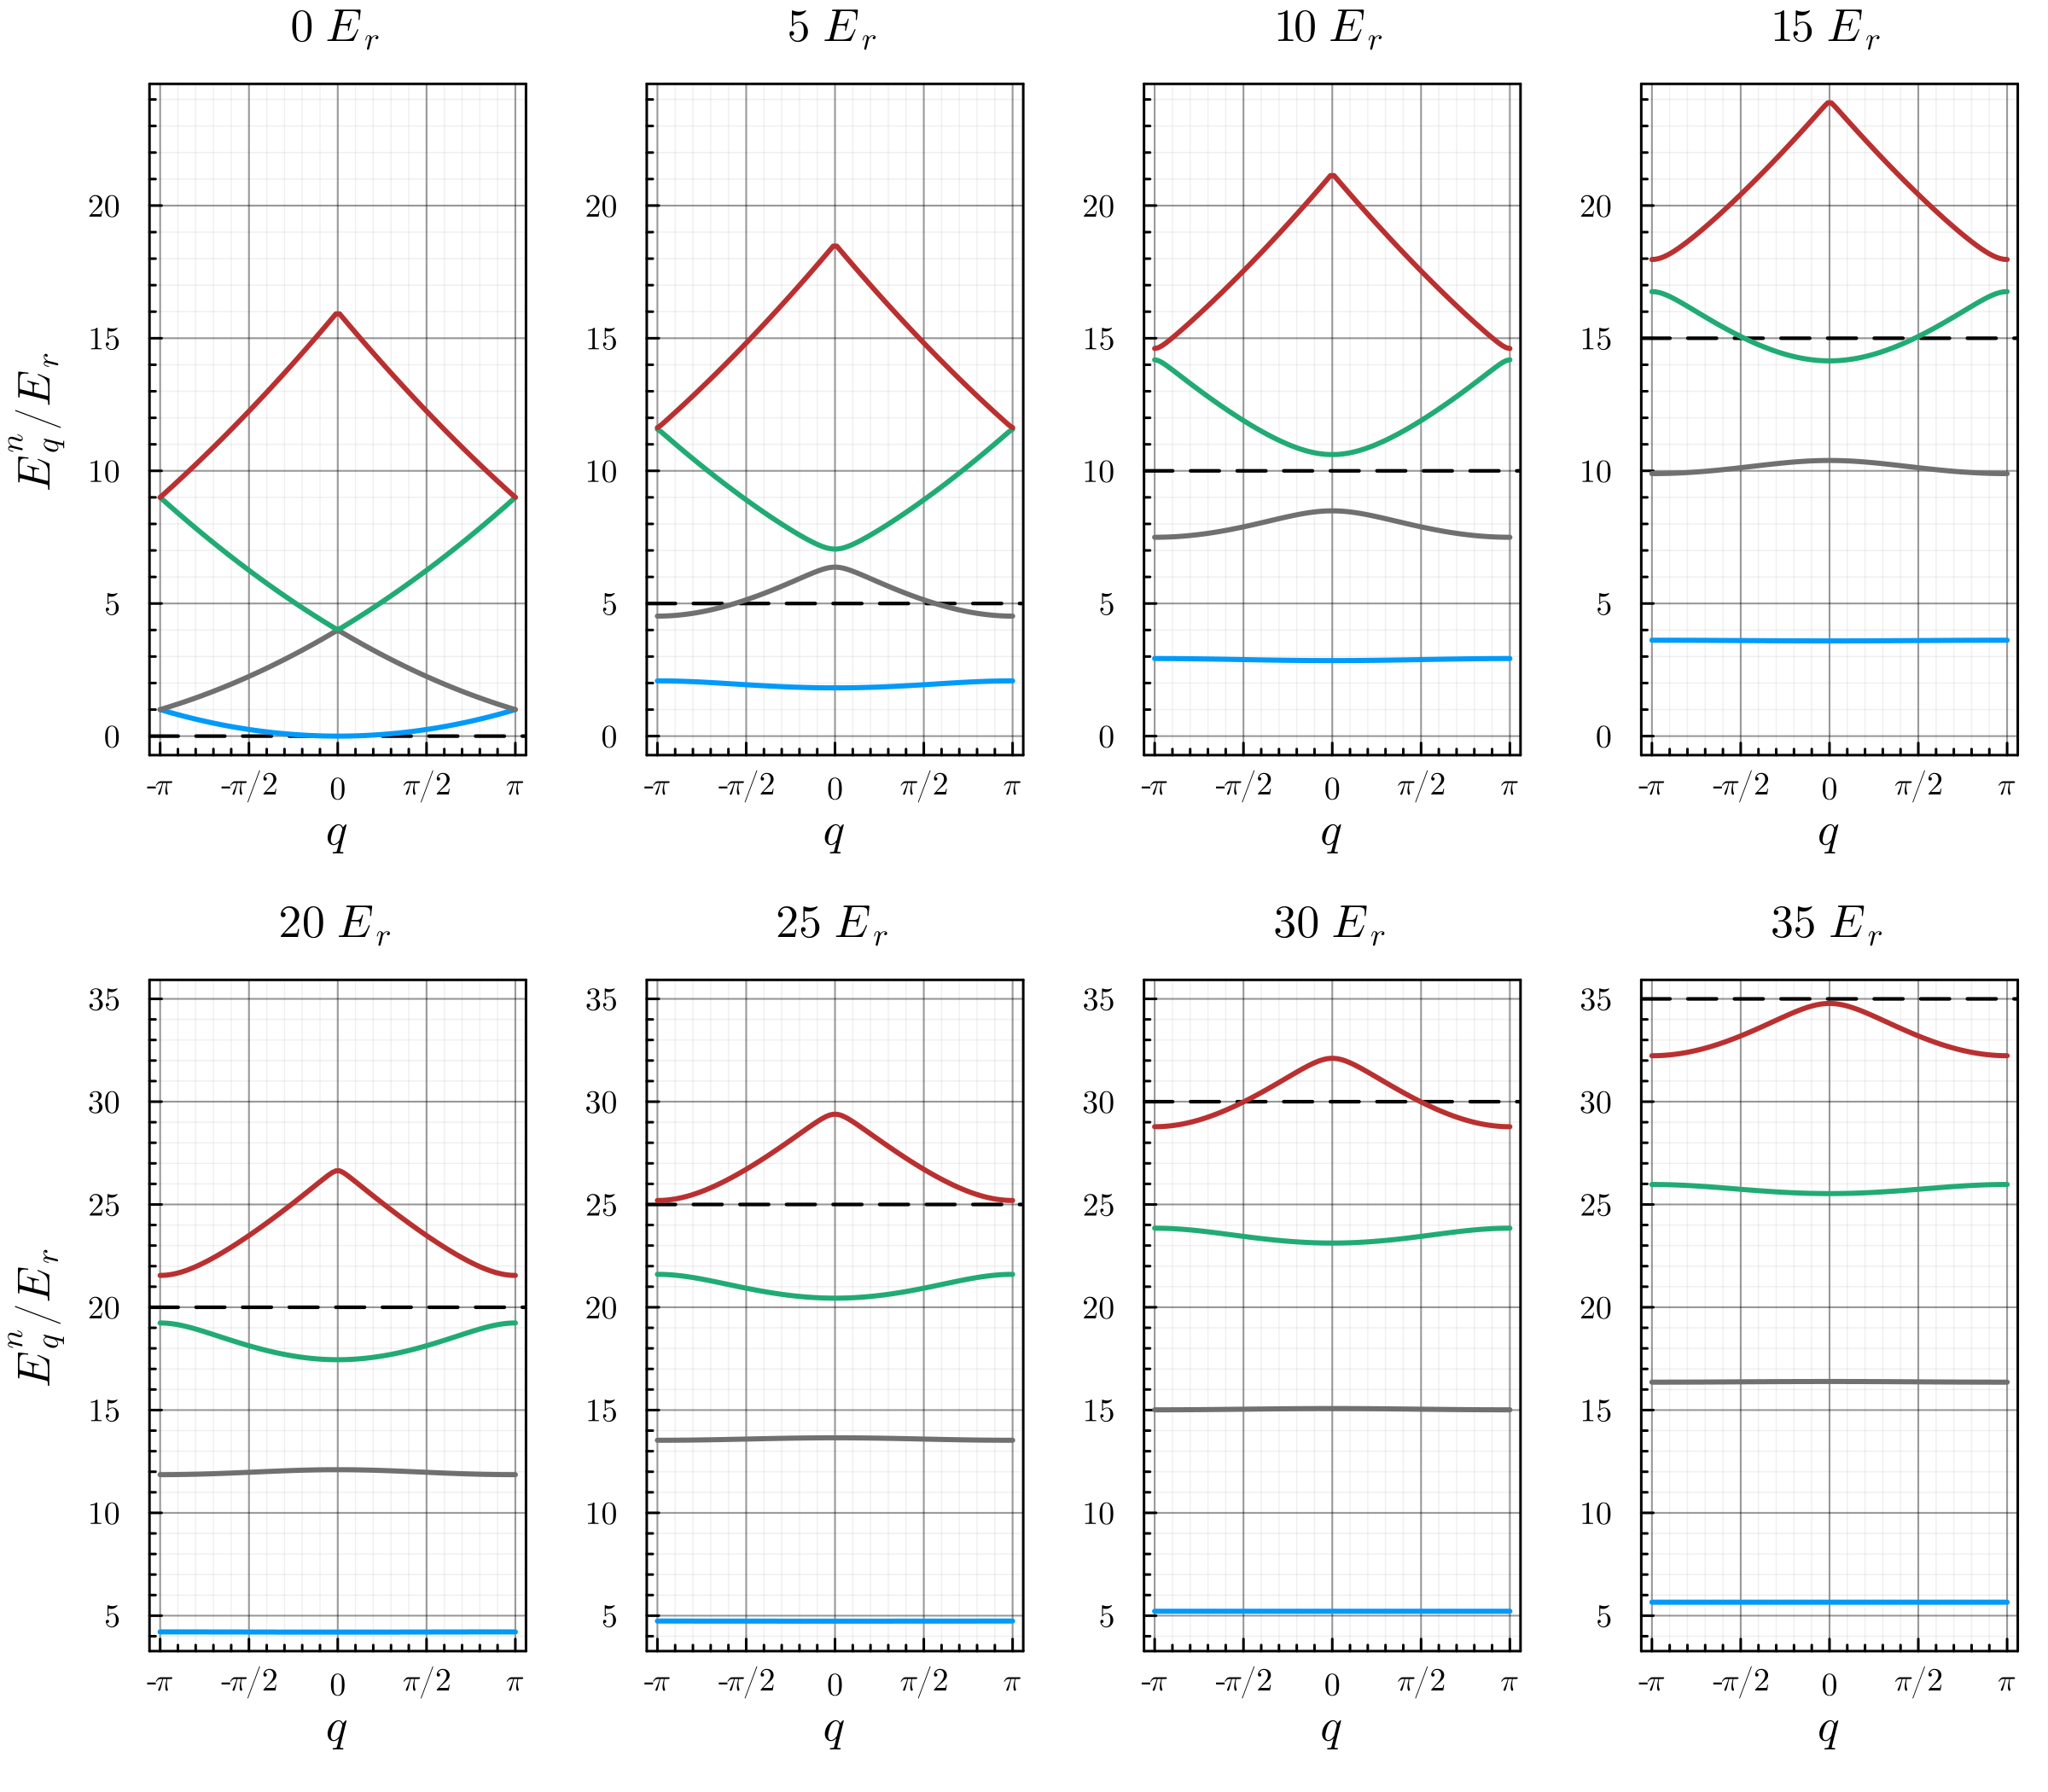
\includegraphics[width=\textwidth]{ch2/energy_bands.png}
    \end{subfigure}
    \caption{First four energy bands of a 1D lattice for various lattice potentials. The black dashed line indicates the lattice depth.}
    \label{fig:bands}
\end{figure}
%%% FIG %%%
\FloatBarrier \!\!\!\!\!\!\!\!\!\!\!

In Fig. \ref{fig:bands} we have plotted the energy bands for the 1D system by diagonalizing the Hamiltonian in the Fourier basis. We see that for the free particle case $(V=0)$, we have the usual parabolic band structure. However, as the lattice potential is increased, band gaps emerge and the widths of the lower bands become smaller, resulting in equally spaced flat bands. This is expected since we can approximate the minima of the periodic potential as a harmonic oscillator for large $V$. 
%%% FIG %%%
\begin{figure}[!htb]
    \centering
    \begin{subfigure}[b]{\textwidth}  %keep total sum <1 to show in same line
        \centering
        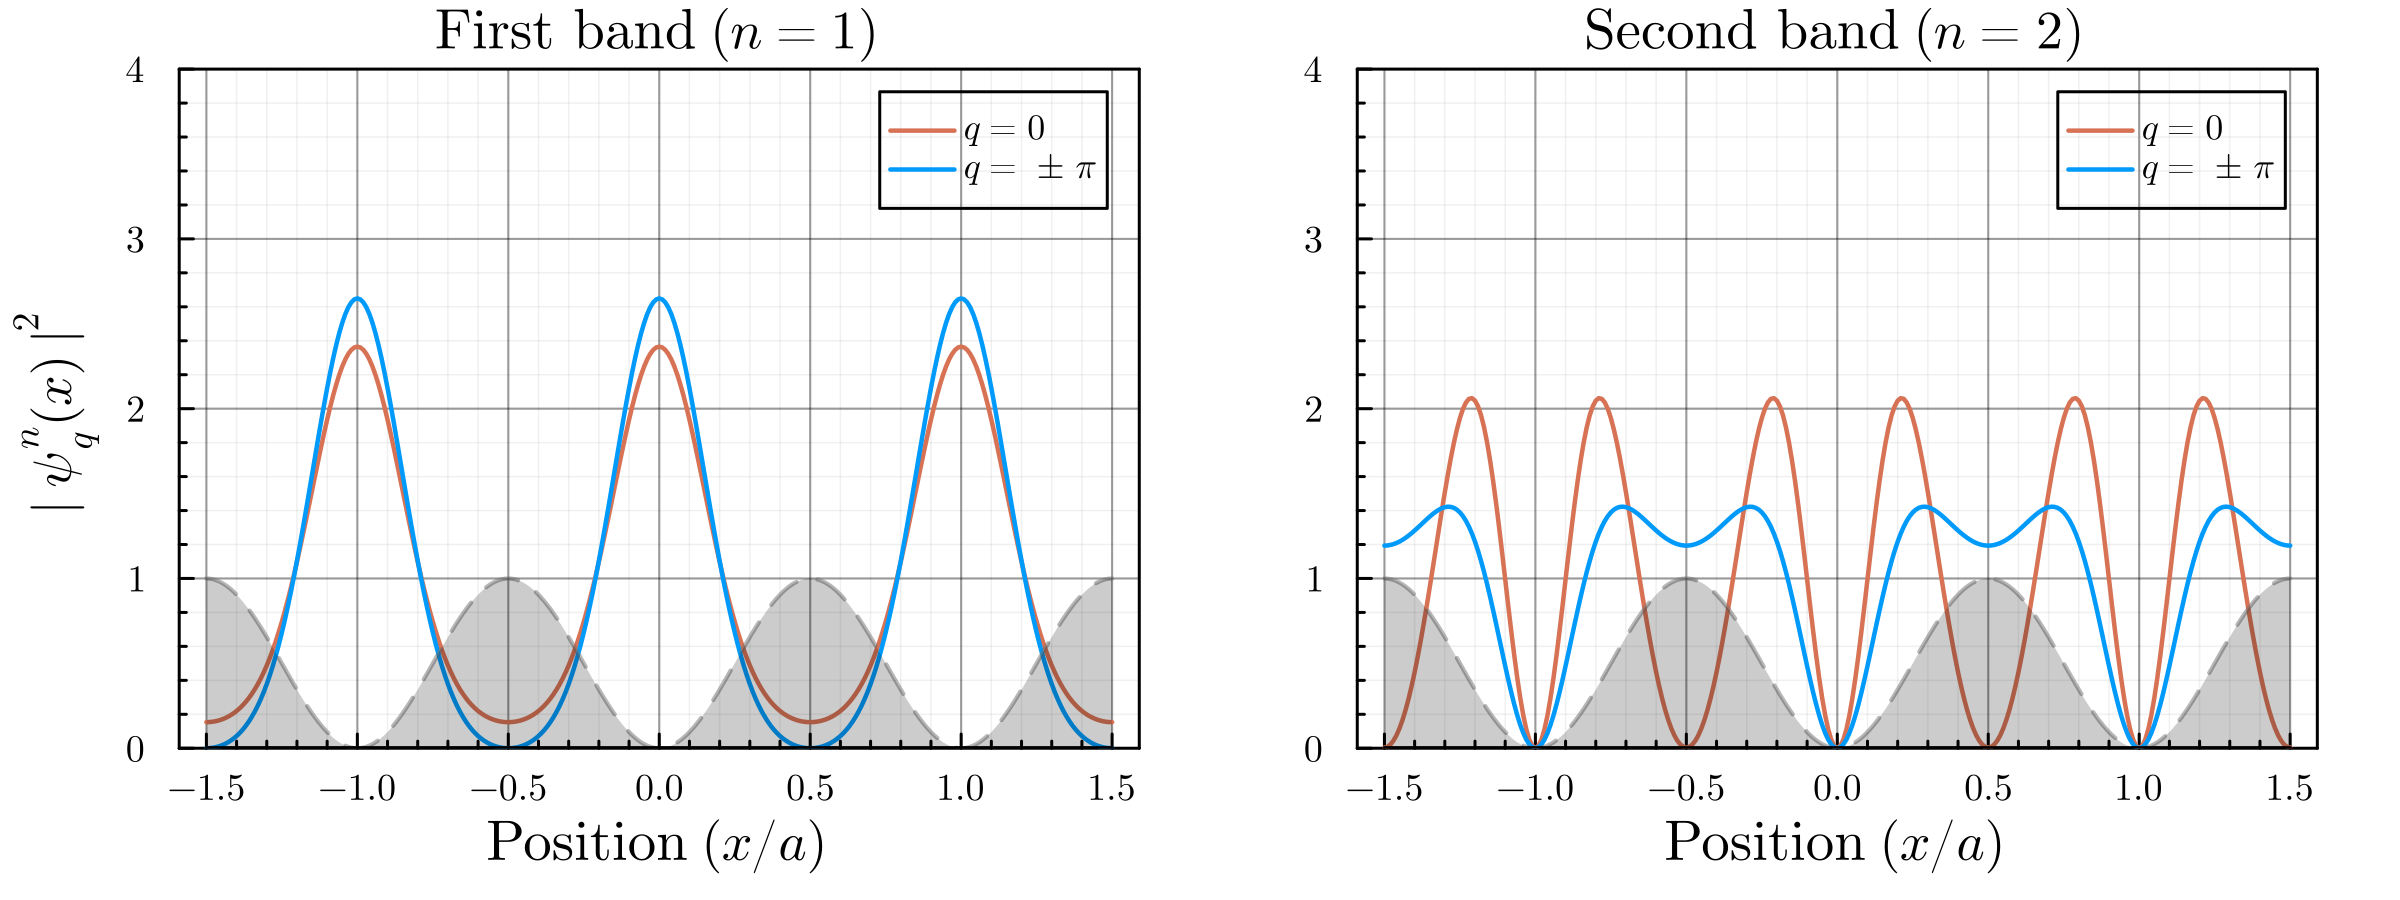
\includegraphics[width=\textwidth]{ch2/bloch_wf.png}
    \end{subfigure}
    \caption{Probability distribution of Bloch wave-functions for $V_0 = 5E_r$. The lattice potential (black) is plotted to indicate the periodicity of the system.}
    \label{fig:bloch}    
\end{figure}
%%% FIG %%%
\FloatBarrier \!\!\!\!\!\!\!\!\!\!\!

\section{Constructing a localized basis}
While the Bloch wavefunctions form a perfectly valid basis set for a periodic system, they are also delocalized across the entire lattice as seen in Fig. \ref{fig:bloch}. Such a situation is rather cumbersome to work with, as will become clear in the next chapter when we discuss the formalism to describe many-particle physics. Instead, we look for a localized basis set.  
\vspace{0.5cm}\\
A simple recipe can be obtained by drawing a parallel with the free-particle case once again. We know that the energy eigenstates are plane waves which are delocalized across all space, and performing a Fourier transformation from $k \to x$ gives us Dirac delta functions, which are highly localized. Similarly, the quasi-momentum $q$ plays the role of $k$ here and by performing a Fourier transform over the first Brillouin zone, we can construct a new basis by introducing a conjugate variable $R$ that is analogous to $x$. 
\begin{equation}
    \phi^n_R(x) = \frac{1}{N}\sum_{q \in BZ} e^{-iqR} \psi_q^n(x)
\end{equation}
where $\psi_q^n(x)$ are the Bloch wave-functions of the $n$th band, $N$ is the number of unit cells in the lattice and $\phi_R^n(x)$ are the so-called \textit{Wannier} functions. An immediate consequence of this procedure is that the Wannier functions are no longer energy eigenstates, but that is a fair price to pay for a localized basis. Also note that $R$ can take the values $na$ where $a$ is the lattice spacing, and $n \in \mathbb{Z}$.
%%% FIG %%%
\begin{figure}[!htb]
    \centering
    \begin{subfigure}[b]{\textwidth}  %keep total sum <1 to show in same line
        \centering
        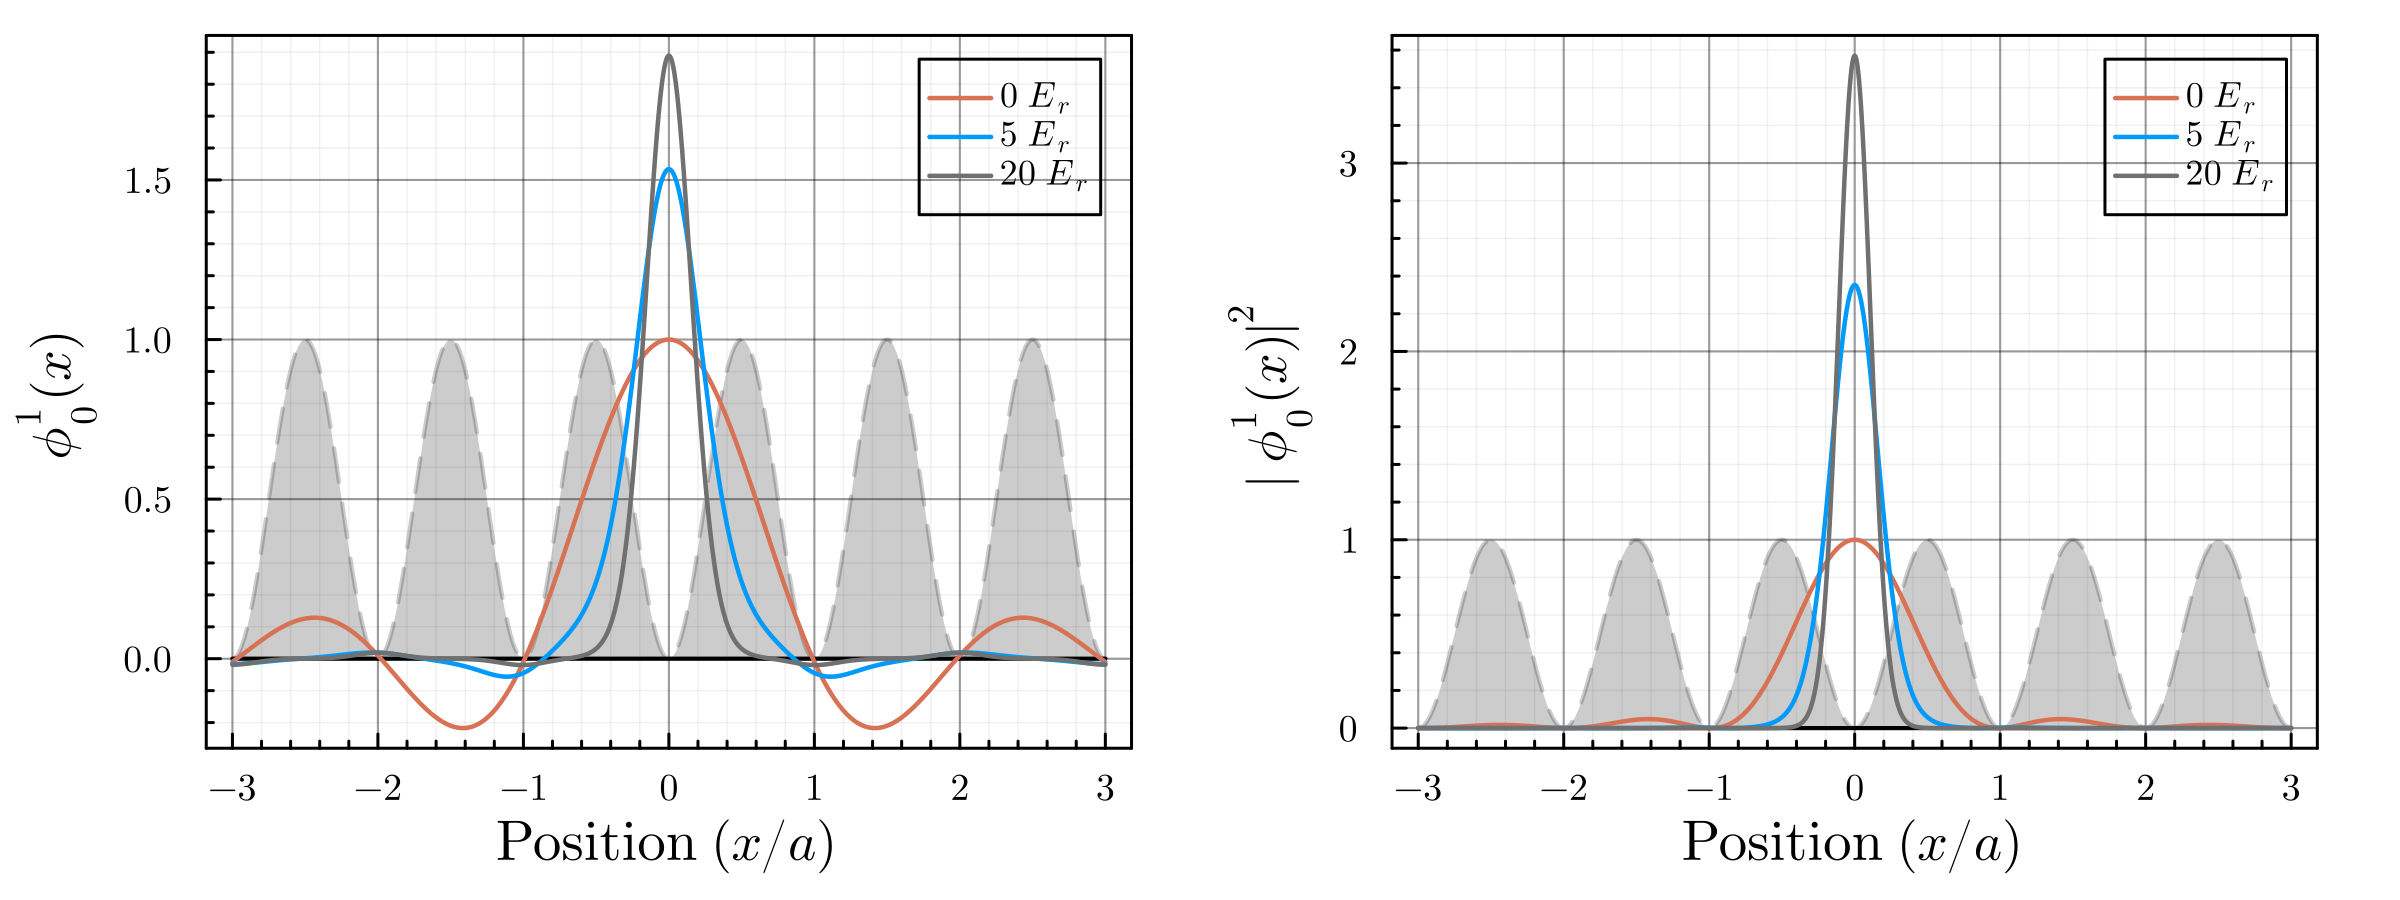
\includegraphics[width=\textwidth]{ch2/wannier_wf.png}
    \end{subfigure}
    \caption{Probability amplitude and density of Wannier wave-functions for Wannier functions of the lowest band. The lattice potential (black) is plotted to indicate the periodicity of the system.}
    \label{fig:wannier}
\end{figure}
%%% FIG %%%
\FloatBarrier \!\!\!\!\!\!\!\!\!\!\!

We see from Fig. \ref{fig:wannier} that as the lattice depth is increased, the Wannier function becomes more localized. In fact, as mentioned earlier, a deep lattice potential can be approximated as a harmonic well and the corresponding Wannier function approaches a gaussian. Let us now try to ascribe meaning to the conjugate index $R$, by considering the following expression for some $m \in \mathbb{Z}$.
\begin{align*}
    \phi_{R+ma}^n(x) &= \frac{1}{N}\sum_{q \in BZ} e^{-iqR} e^{-iqma} \psi_q^n(x)\\    
    &= \frac{1}{N}\sum_{q \in BZ} e^{-iqR} \psi_q^n(x - ma)\\
    &= \phi_{R}^n(x - ma)
\end{align*}
We see that translation in $R$ corresponds to simply shifting the Wannier function in real space by the same amount! This motivates the fact that $R$ is simply an index to label the lattice site on which the Wannier function is localized. 

\subsection{Gauge freedom and non-uniqueness}
At this point, we must bring up a peculiar feature of the Bloch wavefunctions, namely that there exists a gauge freedom in its definition.
\begin{equation}
    \tilde \psi_q^n(x) \equiv e^{i\chi_n(q)} \psi_q^n(x)
\end{equation}
where $\chi_n(q)$ can be any arbitrary function over the reciprocal lattice vectors and cannot be determined from the Schr\"{o}dinger equation. More generally we can describe it in terms of a unitary operation, $U$, like so:
\begin{align}
    \tilde \psi_q^n(x) &= \sum_{m =1}^N U_{mn}^{(q)} \psi_q^n(x)\\
    \phi^n_R(x) &= \frac{1}{N}\sum_{q \in BZ} e^{-iqR} \tilde\psi_q^n(x)
\end{align}
This gauge freedom clearly carries over to the Wannier functions, rendering them non-unique! Luckily, this does not change the fact that any choice of Wannier functions will still be localized, just that they may have different 'shapes'. This motivates the existence of a possibly unique set of Wannier functions that are \textit{maximally localized}\cite{Pavarini2011TheLA}. For instance, such a set may be determined by minimizing the variance of the position operator.
\begin{equation}
    \Omega = \sum_n \langle x^2 \rangle_n  - \langle x \rangle^2_n
\end{equation}
Things can get even more complicated when the energy bands are close enough to intersect, in which case we must allow mixing of the Wannier functions with respect to the $n$ index as well\cite{Marzari_2012, Walters_2013}. However, for the purpose of this thesis, we do not take these complexities into account and simply proceed with the choice of $\chi_n(q) = 0$. This suffices for a rough order of magnitude calculation to motivate the discussions in the following chapters.